%%%%%%%%%%%%%%%%%%%% author.tex %%%%%%%%%%%%%%%%%%%%%%%%%%%%%%%%%%%
%
% sample root file for your "contribution" to a contributed volume
%
% Use this file as a template for your own input.
%
%%%%%%%%%%%%%%%% Springer %%%%%%%%%%%%%%%%%%%%%%%%%%%%%%%%%%


% RECOMMENDED %%%%%%%%%%%%%%%%%%%%%%%%%%%%%%%%%%%%%%%%%%%%%%%%%%%
\documentclass[graybox]{svmult}

% choose options for [] as required from the list
% in the Reference Guide

\usepackage{mathptmx}       % selects Times Roman as basic font
\usepackage{helvet}         % selects Helvetica as sans-serif font
\usepackage{courier}        % selects Courier as typewriter font
\usepackage{type1cm}        % activate if the above 3 fonts are
                            % not available on your system
%
\usepackage{makeidx}         % allows index generation
\usepackage{graphicx}        % standard LaTeX graphics tool
                             % when including figure files
\usepackage{multicol}        % used for the two-column index
\usepackage[bottom]{footmisc}% places footnotes at page bottom

\usepackage[sort&compress,numbers]{natbib}
\usepackage{todonotes}
\usepackage{amsmath, amsfonts}
\usepackage{blkarray}
\usepackage{xypic}

%% macros for the manuscript.... %%%%%%%%%%%%%%%%%%%%%%%%%%%%%%%%%%%%%%%%%%%

\newcommand{\partition}{\ensuremath{\mathbf{P}}}

%% Symbols for likelihoods
\newcommand{\G}{\ensuremath{G}}
\renewcommand{\D}{\ensuremath{D}}
\renewcommand{\lhd}{\ensuremath{\mathcal{L}}}
\newcommand{\T}{\ensuremath{T}}
\renewcommand{\E}{\ensuremath{E}}

\newcommand{\argmax}{\ensuremath{\operatorname*{arg\,max}}}
\newcommand{\intd}{\ensuremath{\mathrm{\;d\,}}}

\newcommand{\trans}[3]{\ensuremath{#1 \xrightarrow{#2} #3}}

%%%%%%%%%%%%%%%%%%%%%%%%%%%%%%%%%%%%%%%%%%%%%%%%%%%%%%%%%%%%%%%%%%%%%%%%%


% see the list of further useful packages
% in the Reference Guide

\makeindex             % used for the subject index
                       % please use the style svind.ist with
                       % your makeindex program

%%%%%%%%%%%%%%%%%%%%%%%%%%%%%%%%%%%%%%%%%%%%%%%%%%%%%%%%%%%%%%%%%%%%%%%%%%%%%%%%%%%%%%%%%

\begin{document}

\title*{Ancestral population genomics with coalescent hidden Markov models}
\author{Jade Yu Cheng and Thomas Mailund}
\institute{Jade Yu Cheng \at FIXME
	\email{name@email.address}
\and Thomas Mailund \at Bioinformatics Research Centre, Aarhus University \email{mailund@birc.au.dk}}
\maketitle

\abstract{FIXME}


\section{Introduction}

Understanding how species form and diverge is a central topic of biology and by observing emerging species today we can understand many of the genetic and environmental processes involved. Through such observations we can understand the underlying forces that drive speciation, but in order to understand how specific speciations occurred in the past, and understand the specifics of how existing species formed, we must make inference from the signals these events have left behind. The study of fossils is a powerful approach here, but not the only avenue to study past speciations; the speciation processes leave fossils in the genome of the resulting species, and through what you might call genetic archaeology we can study past events from the signals they left behind.

Over the last three decades several inference methods were developed to model speciation and estimate the timing of splits, the presence or absence of gene-flow during a split, and estimate population genetics parameters of the ancestral species, such as the effective population size. For a detailed review of these, focusing on the human/chimpanzee speciation, we refer to~\citet{Mailund:2014fyb}.

Early methods considered short aligned segments and modelled how these would be different samples from the underlying coalescence process in the ancestral species~\cite{Takahata:1995kl, Innan:2006hc, Burgess:2008kf, Rannala:2003vt, Yang:2002wz, Yang:2006eu, Yang:2010fm, Becquet:2009hta, Chen:2001dka, Wall:2003vb}. Common for these is that recombination was not explicitly modelled, with the exception of the model of~\citet{Becquet:2009hta} that allows intra-locus recombination at a cost in computational complexity. The methods considered genomic regions sufficiently short that recombination was considered unlikely and sufficiently apart that the regions could be considered independent.

Sequencing technology, however, has progressed dramatically over the last decade and now multiple full genome sequences are readily available for many related species and constructing sequences for new species is affordable for even small research groups. To fully exploit such data, models will have to explicitly consider recombination. We have to move from ancestral population genetics to \emph{genomics}.


\subsection{The sequential Markov coalescent and coalescent hidden Markov models}

Models for ancestral population genetics are based on coalescence theory~\cite{Hein:2004ta} that describes the stochastic process of how lineages of a present day sample coalesce into common ancestors back in time. The outcome of this process, when both coalescence events and recombination events are considered, is called the \emph{ancestral recombination graph} or ARG. The coalescence process with recombination was originally described as a process running backward in time, but~\citet{Wiuf:1999gua} showed that it could also be modelled as a process running along a sequence alignment. This process, however, is computationally intractable for long sequences because it requires keeping track of all local gene trees along the sequence.

Considering the coalescence process as a sequential process along a sequence alignment lead to two innovations for modelling long sequence alignments experiencing recombination: the \emph{sequential Markov coalescence} and \emph{coalescent hidden Markov models}; two ideas that while starting out from different ideas have now largely merged.

The sequential Markov coalescence was introduced by~\citet{McVean:2005hoa} who considered a coalescence process where lineages are not allowed to coalesce unless they share ancestral material. They showed that this process would be Markov when considered as a sequential process and dubbed the process the sequential Markov coalescence, SMC. Because the model originated from restrictions on which lineages could coalesce, rather than an attempt to approximate the Wiuf \& Hein model as a Markov process, it does not allow two lineages resulting from a recombination to re-coalesce unless they have first coalesced with other lineages. Consequently, when there are few lineages a large fraction of the coalescence event that would be allowed in the coalescence process are not allowed in the SMC. This was amended by~\citet{Marjoram:2006hpa} in a model named SMC$^\prime$ that matches the SMC process except for explicitly allowing these back-coalescence events. This model was further extended to allow higher order Markov dependencies in the MaCS model by \citet{Chen:2009fga}. This early work on sequential Markov coalescence models focused on simulating sequence data and not on data analysis.

Independently of the work on sequential Markov coalescent models we developed a model for inferring the speciation dates of the human-chimpanzee and human-gorilla splits in \citet{Hobolth:2007gza}. While this model was based on ideas from \citet{Wiuf:1999gua}, combined with ideas from \citet{Takahata:1995kl}, it did not explicitly model the coalescence process. Instead it simply specified a hidden Markov model with gene genealogies as hidden states and fitted the rate of changes in these to a sequence alignment. Parameters from the coalescence process were then inferred based on the fitted hidden Markov model parameters. The term \emph{coalescent hidden Markov model}, or CoalHMM, was coined in this paper.

We later constructed a model that merges the coalescent hidden Markov model from \citet{Hobolth:2007gza} with the SMC model in \citet{Dutheil:2009dta}. This model was also applied to the human-chimpanzee and human-gorilla speciation and revealed very clearly that not allowing back-coalescences in the long time periods where all sequences are in isolated species would lead to a serious underestimation of the recombination rate.

To alleviate this we developed a new model that uses continuous time Markov chains (CTMCs) to explicitly model all recombination and coalescence events possible for a pair of neighbouring nucleotides and built a CoalHMM from this in \citet{Mailund:2011dva}. As an added benefit, this model allowed us to infer parameters from a pair of sequences, where the previous methods requires three sequences and incomplete lineage sorting between them.

Independent of this, Li \& Durbin developed a CoalHMM based on the SMC for pairs of sequences, the so-called pairwise sequential Markov coalescent model PSMC~\cite{Li:2011eza}, for inferring changing effective population sizes back in time. \citet{Paul:2010iba} and \citet{Paul:2011gva} developed a model combining the SMC with a conditional sampling approach to scale the data size beyond pairs, while \citet{Rasmussen:2014cqa} developed a sampling approach with the same aim.

A number of models followed these, extending the models to consider gene-flow patterns~\cite{Steinrucken:2013kba,Mailund:2012ewa}, changing population sizes~\cite{Sheehan:2013iba,Schiffels:2014cua} or inference of recombination patters, and selection \cite{Munch:2014cba, Munch:2014cwa}, \cite{Dutheil:2015kl, Munch:2016dn}, and CoalHMMs have been used in a number of whole genome analyses \cite{Locke:2011gna, Hobolth:2011dia, Scally:2012ika, Prufer:2012ea, Miller:2012cxa, Abascal:2016cy, PradoMartinez:2013dna, Jonsson:2014fga}.

In this chapter we will present the theory underlying our approach to constructing coalescent hidden Markov models and present our current implementations of various models and how you can apply these to your own genomic analyses.

\section{The hidden Markov model approximation to the coalescent with recombination}

The main objectives of the methods we describe in this chapter is to infer demographic parameters, $\Theta$, given genetic data, $D$. In particular, we are interested in computing the likelihood of parameters given data, $\lhd(\Theta\,|\,D)$. Here, we assume that the genetic data is aligned sequences of a number of sampled genes. If our samples were related through a known tree, $\G$, this would be a solved problem. There are standard approaches, as Felsenstein's peeling algorithm \cite{Felsenstein_1981}, to computing the probability of seeing a particular alignment given a genealogy and a substitution model, which we could subsume into the parameters $\Theta$.

Of course, we never know the exact tree relating a sample of genes, but with a density over genealogies, $f(\G\,|\,\Theta)$, we could treat $\G$ as a nuisance parameter and integrate it away to get
\begin{equation}
    \lhd(\Theta\,|\,\D) = \int f(\D\,|\,\G,\Theta) f(\G\,|\,\Theta) \intd\G .
\end{equation}

If we consider a single column of the genetic data, then we know that our samples are related through some tree. With more than one nucleotide, we cannot know this---recombinations could have broken apart ancestral lineages and different nucleotides along the alignment might be related through different genes. The real genealogy underlying genetic sequence data is a graph, known as the \emph{ancestral recombination graph} \cite{Hein:2004ta}.\todo{Should we have an example of an ARG?}

We usually assume that, although the genealogies at different sites are not independent, the mutations at these sites are, so we could break down $\Pr(\D\,|\,\G,\Theta)$ into alignment columns and get
\begin{equation}
  \Pr(\D\,|\,\G,\Theta) =
  \prod_{i=1}^L \Pr(\D_i\,|\,\G_i,\Theta)
\end{equation}
where $\D_i$ denote the column $i$ in the alignment and $\G_i$ the (local) genealogy at site $i$. This gives us the parameter likelihood
\begin{equation}
	\label{eq:likelihood-integral}
    \lhd(\Theta\,|\,\D) = 
    \int \prod_{i=1}^L \Pr(\D_i\,|\,\G_i,\Theta) f(\G\,|\,\Theta) \intd\G .
\end{equation}

The density over genealogies is available from coalescence theory and theoretically we could do this integral. In practice, however, the space of possible genealogies makes this approach intractable.

The sequential Markov coalescence approximates the coalescence process with recombination by assuming that the dependencies between genealogies is Markov:
\begin{equation}
  \label{eq:markov-genealogy}
  f(\G\,|\,\Theta) \approx
  f(\G_1\,|\,\Theta)\prod_{i=2}^{L}f(\G_{i}\,|\,\G_{i-1},\Theta)
  .
\end{equation}

With this approximation, the joint density of data and genealogies become
\begin{equation}
  \label{eq:coalhmm-joint-probability}
  f(\D,\G\,|\,\Theta) = 
  	f(\G_1\,|\,\Theta)
  	\prod_{i=2}^{L}f(\G_{i}\,|\,\G_{i-1},\Theta)
  	\prod_{i=1}^L \Pr(\D_i\,|\,\G_i,\Theta)
  	,
\end{equation}
which is characteristic of \emph{hidden Markov models}, stochastic models of sequences formulated as joint probabilities of a \emph{hidden} sequence $\mathbf{Z}=(Z_1,Z_2,\ldots,Z_L)$ and an \emph{observed} sequence $\mathbf{X}=(X_1,X_2,\ldots,X_L)$ where the dependencies between the hidden states, $Z_i$, is Markov and the observed states, $X_i$, are independent conditional on the hidden states, and the joint probability is
\begin{align}
  \Pr(\mathbf{X},\mathbf{Z})
    &= 
  	\Pr(Z_1)
  	\prod_{i=2}^{L}\Pr(Z_{i}\,|\,Z_{i-1})
  	\prod_{i=1}^L \Pr(X_i\,|\,Z_i)
  	\\
    \label{eq:hmm-joint-probability}
  	&=
  	\pi_{Z_1}
  	\prod_{i=2}^{L}\T_{Z_{i-1},Z_{i}}
  	\prod_{i=1}^L  \E_{Z_i,X_i}
\end{align}
where in \eqref{eq:hmm-joint-probability} $\pi$ denotes a vector of \emph{initial state probabilities}, $\T$ a matrix of \emph{transition probabilities}, and $\E$ a matrix of \emph{emission probabilities}.\footnote{The intuition is that the $\mathbf{Z}$ sequence is not observed but each $Z_i$ emits a symbol, $X_i$ that \emph{is} observed.}

The form of \eqref{eq:coalhmm-joint-probability} closely resembles \eqref{eq:hmm-joint-probability} except that the matrix representation for the hidden Markov model requires the state space to be finite, which the set of all possible local coalescent genealogies is not. The branch lengths of genealogies are real numbers, thus there are infinitely many genealogies. To approximate the coalescent with recombination we employ another approximation and discretise time. We divide the real line into $m$ time points and require that all coalescence event occur in one of those.

Constructing hidden Markov models therefore consist of constructing the initial state probability vector
\begin{equation}
  \label{eq:initial_prob}
  \pi_{\G_1} = \Pr(\G_1\,|\,\Theta),
\end{equation}
the transition probability matrix
\begin{equation}
  \label{eq:transition_prob}
  \T_{\G_{i-1},\G_i} = \Pr(\G_i\,|\,\G_{i-1},\Theta),
\end{equation}
and the emission probability matrix
\begin{equation}
  \E_{\G_i,\D_i} = \Pr(\D_i\,|\,\G_i,\Theta)
\end{equation}
to capture as well as possible under the approximation the probabilities we would see given the parameters $\Theta$. (In \eqref{eq:initial_prob} and \eqref{eq:transition_prob} we have replaced densities, $f(-)$, with probabilities, $\Pr(-)$, to indicate that we have discretised the set of genealogies).

The emission probabilities can be computed using standard substitution models and algorithms, and we will not describe this further. For the initial states and transition probabilities we get these from the joint probability of two neighbouring genealogies, $\Pr(\G_i,\G_{i+1})$ (where we assume that the Markov model in \eqref{eq:markov-genealogy} is homogeneous and this probability thus the same for all $i$). From this joint probability we can marginalise and get
\begin{equation} \label{eq:pi-from-joint-prob}
  \Pr(\G_i) = \sum_{\G_{i+1}} \Pr(\G_i,\G_{i+1})
\end{equation}
and we set $\pi_{\G_1}=\Pr(\G_1)$ and 
\begin{equation} \label{eq:transitions-from-joint-prob}
  \T_{\G_{i-1},\G_i} = \frac{\Pr(\G_{i-1},\G_i)}{\Pr(\G_{i-1})}.
\end{equation}

The crux of the construction is thus computing $\Pr(\G_i,\G_{i+1})$, which we describe in the next section.

An important point to make first, however, is that by formulating the model as a hidden Markov model we obtain a number of efficient algorithms for parameter estimation and for decoding the most likely hidden genealogies. For example, to compute the likelihood of the model, the discretisation changes the integral from \eqref{eq:likelihood-integral} to the sum
\begin{equation}
  \label{eq:likelhood-sum}
  \lhd(\Theta\,|\,\D) = 
  \sum_{\G=(\G_1,\G_2,\ldots,\G_L)} 
  	\left[
   	  \pi_{\G_1}
  	  \prod_{i=2}^{L}\T_{\G_{i-1},\G_{i}}
  	  \prod_{i=1}^L  \E_{\G_i,\D_i}
  	\right]
\end{equation}
which in this form involves summing over a sum with an exponential number of terms as a function of $L$, but which can be computed in time $O(N^2L)$ using dynamic programming, where $N$ is the number of hidden states, i.e.\ the number of genealogies. The algorithm, known as the \emph{forward} algorithm, defines $F(g,i)$ to be the probability of being in genealogy $g$ at index $i$ and having observed $(\D_1,\ldots,\D_i)$. This function can be computed recursively
\begin{equation}
  F(g,i) = 
  \begin{cases}
  	\pi_g & i = 1 \\
  	\E_{g,\D_i} \times \sum_{\G_{i-1}}\T_{\G_{i-1},g} \times F(\G_{i-1},i-1)
  	& \mathrm{otherwise}
  \end{cases}
\end{equation}
and the recursion can be replaced by dynamic programming, where we fill a table \texttt{F} with $\mathtt{F}[g,1] = \pi_g$ for all $g$ and then from $i=2$ to $i=L$ compute
\[
\mathtt{F}[g,i] = \E_{g,\D_i} \times \sum_{\G_{i-1}}\T_{\G_{i-1},g} \times \mathtt{F}[\G_{i-1},i-1]
\]
for all $g$. The \texttt{F} table has $N\times L$ entires and computing each recursive entry requires a sum over $N$ elements, giving us a running time of $O(N^2L)$. Once \texttt{F} has been filled, we can get the likelihood by summing over all final genealogies:
\begin{equation}
  \lhd(\Theta\,|\,\D) = \sum_{g} \mathtt{F}[g,L].
\end{equation}

Thus, to get a tractable approach to infer demographic parameters from genetic data under the coalescence with recombination, we only need to construct the three HMM parameters $\pi$, $\T$, and $\E$. As seen in \eqref{eq:pi-from-joint-prob} and \eqref{eq:transitions-from-joint-prob}, we can derive $\pi$ and $\T$ from joint probabilities of two genealogies, and as mentioned earlier, we can compute $\E$ from standard algorithms (once we have discretised time).

\section{Constructing CoalHMMs}

The crux of deriving a CoalHMM is computing probabilities $\Pr(G_i,G_{i+1})$ in discretised time. We will show how to do this in three steps. First we show how to construct models that trace the ancestry of neighbouring nucleotides back in time. The models we build this way captures fixed demographic scenarios and we can only use them to infer parameters from such. To allow changes in the ancestry, such as populations splitting and merging, we need a way to combine the models, and we describe this secondly. The CTMCs we develop for the coalescence processes contain more information than is captured by genealogies, and the final step in constructing CoalHMMs involve integrating over this extra hidden information after discretising time.

\subsection{The coalescent process and continuous time Markov chains}

The sequential Markov coalescent and coalescent hidden Markov models aim to approximate the coalescent model with recombination in order to make analysis tractable. The coalescent model of population genetics describes the ancestry of a sample of observed genes and gives probabilities to all the possible genealogies that can explain the observation. The typical formulation of the model is as a continuous time Markov chain (CTMC) that describes how the sampled genes find common ancestors as we look further and further back in time. 

A (time homogeneous) continuous time Markov chain (CTMC) is a random process $\{\,X(t) \;|\; t \geq 0 \,\}$ where the infinitesimal rate of change between states at time $t$ is given by a \emph{rate matrix} $Q$: Let $\pi(t)$ be the vector of state probabilities $\pi(t)_i = \Pr(X(t)=i)$ then $\frac{\mathrm{d}\,\pi(t)}{\mathrm{d}\,t} = \pi(t)^TQ$. The off-diagonal entries of $Q$ contains the rates at which the system changes state, so $Q_{i,j}$ is the rate of change from state $i$ to state $j$, and the diagonal entries are given by $Q_{i,i} = - \sum_{j\neq i} Q_{i,j}$. The probability of going from state $i$ at time $s$ to state $j$ at time $t>s$ in such a system is given by $\Pr(X(t)=j\,|\,X(s)=i) = \left[\exp\left(Q\left(t-s\right)\right)\right]_{i,j}$ and given an initial probability vector $\pi(0)$ the probability vector at time $t\geq 0$ is given by $\pi(t)^T=\pi(0)^T\exp(Qt)$.

\todo[inline]{Add an example here to make it more understandable.}

There is a rich theory for CTMCs so expressing systems in terms of these gives us a very powerful framework to work in. The key property we will use is the way of computing the transition probabilities $\Pr(X(t)=j\,|\,X(s)=i)$ using matrix exponentiation $\exp\left(Q\left(t-s\right)\right)$. This can be done fully automatically---several algorithms exists and matrix exponentiation is implemented in many numerical software packages \cite{Moler2003}---and it greatly simplifies the mathematical modelling---see e.g.\ \citet{Hobolth:2011hl} and \citet{Andersen:2013iz} for examples of where matrix exponentiation simplifies otherwise rather complex computations.

Constructing a CTMC consists of specifying the rate matrix $Q$ and the initial probability vector $\pi(0)$. In most cases this is relatively straightforward, mathematically at least; explicitly specifying the rate matrix can be problematic when the state space is very large. When the state space is large it becomes necessary to automatically generate it and construct the rate matrix. In the remainder of this section, we describe how to automatically construct CTMCs capturing the coalescence process and how these can then be used to construct coalescent hidden Markov models.

\subsubsection{A token game for constructing CTMCs}

To define a continuous time Markov chain, you need to specify its rate matrix, $Q$, and initial state probabilities, $\pi(0)$. Doing this manually is straightforward for small systems, but infeasible once the state space of the CTMC grows beyond a few tens of states. When developing the CoalHMM in \citet{Mailund:2011dva}, it took us several tries to get it right, and we didn't manage completely until we automated it. The CTMC used in that model has 16 states. The CTMCs we use when constructing CoalHMMs are all constructed automatically from a demography specification, and in this section we explain one formal way of specifying CTMCs that we will use for the remainder of the chapter. The approach is based on \emph{Coloured Petri Nets}~\cite{Jensen:2013jg}, but simplified somewhat since we only need very simple models.

We construct CTMCs by playing a simple game. We imagine we have a bucket, and in this bucket we have a number of ``tokens'', pieces of information we can manipulate. The content of the bucket is a state the CTMC can be in, and the state space of the CTMC is given by the set of states we can reach by manipulating the content of the bucket using a set of transitions---which we will soon make more formal---from a select set of initial states. For coalescence processes, we always start from a single initial state which contain present day genes, the transitions are the events that can happen as we trace the ancestry of these genes back in time, and an instance of this ``token game'' from the initial state until all present day genes have found a common ancestor corresponds to a genealogy of the genes. Thus, our vector $\pi(0)$ is always specified as having a point probability at this initial state and having zero probability everywhere else.

Graphically, we represent the bucket as a circle with the tokens in it. The actual representation in an implementation will be as a set or multi-set, but this graphical representation makes the content of the bucket clearer. An example is shown in Fig.~\ref{fig:example-CPN} of a bucket containing four tokens, the numbers $1$ to $4$.

\begin{figure}[h]
\sidecaption
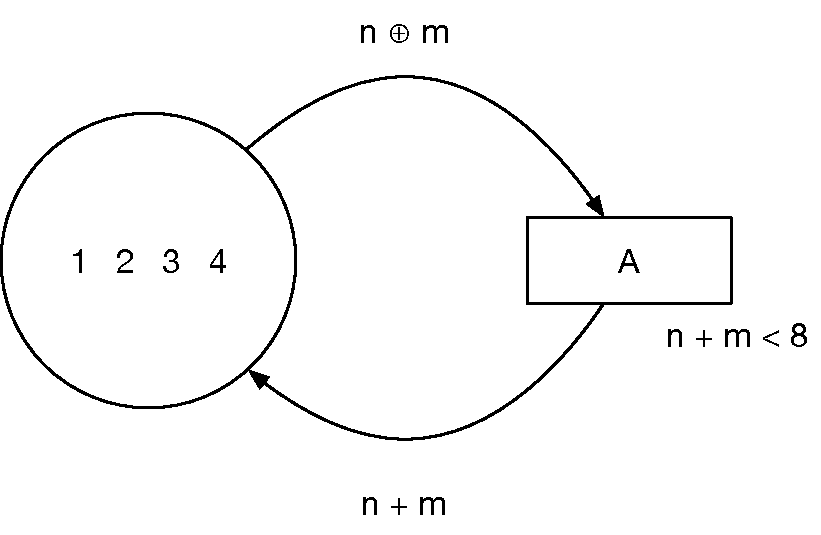
\includegraphics[scale=.45]{figures/example-CPN}
\caption{Example token game that adds together numbers as long as the result is less than eight. The single transition picks up two tokens with rate $A$ and puts back a token that contains the sum of the two. The condition for applying the transition insists that this result must be less than eight.}
\label{fig:example-CPN}
\end{figure}

We represent transitions as boxes. Inside the boxes, we specify the rate at which we can apply them, in Fig.~\ref{fig:example-CPN} we have a single transition that is applied at rate $A$. Transitions will have an edge going from the bucket to the transition and another going back. The edge from bucket to transition specifies which tokens it will pick up from the bucket and the other which tokens it will put back. If it picks up or puts back more than one token, they are written separated by the symbol $\oplus$. The transition in Fig.~\ref{fig:example-CPN} picks up two tokens, named $n$ and $m$ and puts back a single token containing their sum, $n+m$. If their are restrictions to when we can apply a transition, we write those next to the transition. In the case of the addition transition, we require that $n + m < 8$.

Occasionally, we will define transitions textually instead of graphically. In that case, we will write them as an arrow between the input tokens and output tokens with the rate above the error and the condition written afterwards. The $A$ transition from Fig.~\ref{fig:example-CPN} would thus be written ``$\trans{n\oplus m}{A}{n+m}$ when $n+m>8$''.

From the token game we can make a \emph{reachability} or \emph{state space} graph. This graph will contain as its notes all the bucket configurations it is possible to reach by applying the transitions from a set of initial states---or in our case, a single initial state. Whenever we can get from one bucket configuration to another by applying a single transition, we add an edge between the two corresponding graph nodes. We annotate these edges with the rate of the transition---and in cases where there is more than one way to get from one specific node to another, we annotate the edge with the sum of rates at which we can move. Figure~\ref{fig:example-state-space-graph} shows this graph for the token game in Fig.~\ref{fig:example-CPN}. To simplify the notation, we have not labelled the edges with rate $A$ but only the two with $2A$. If an edge does not have a label, think of it as labelled with $A$.

\begin{figure}[t]
\sidecaption[t]
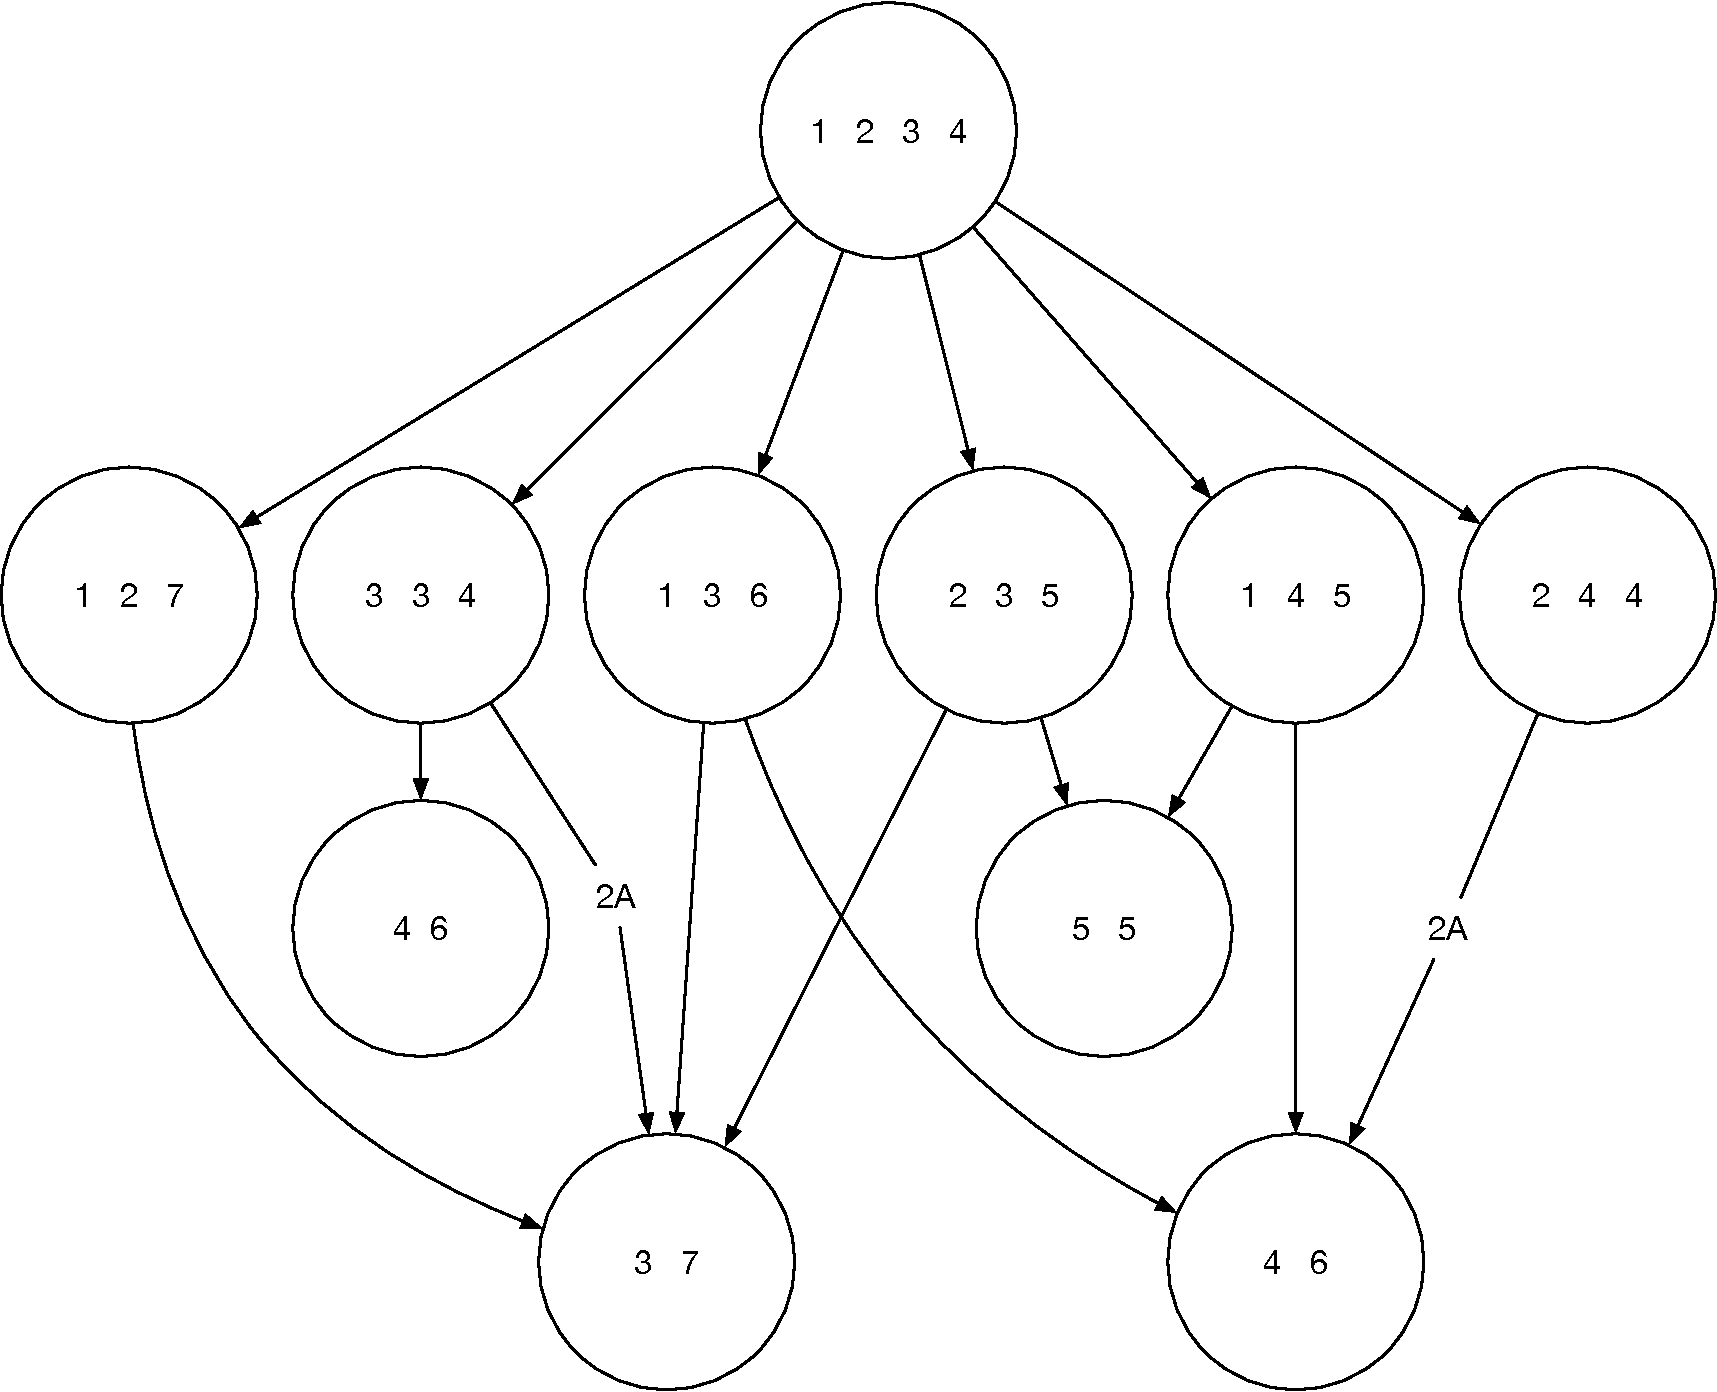
\includegraphics[scale=.30]{figures/example-state-space-graph}
\caption{Example token game that adds together numbers as long as the result is less than eight. The single transition picks up two tokens with rate $A$ and puts back a token that contains the sum of the two. The condition for applying the transition insists that this result must be less than eight.}
\label{fig:example-state-space-graph}
\end{figure}

The final step of constructing the CTMC, getting the rate matrix $Q$ from this graph, is now straightforward. We first enumerate all the nodes, so we have a mapping from CTMC states to matrix indices, and then we construct a matrix $Q$ where we set $Q_{ij}, i\neq j$ to zero if there is not an edge from state $i$ to $j$ in the graph and the rate on the edge if there is. Finally, we set the diagonal elements $Q_{ii}$ to $-\sum_{j \neq i} Q_{ij}$.



\subsubsection{The coalescence process}

The coalescence process \cite{Hein:2004ta} models the genealogy of a set of present day genes by tracking their ancestry back in time. It is constructed as a continuous time Markov chain that runs backwards in time. In its simplest form, there is a single possible transition, a \emph{coalescence} event, that takes two genetic lineages and merge them into one ancestral lineage. Any run of this CTMC from the initial state to a final state, where all present day genes have found their common ancestor, corresponds to a genealogy. Conversely, we can assign probability densities to all genealogies, since the probability of seeing any given genealogy is the same as the probability that the CTMC will have a run matching it.

In the token game formulation of this process, we can represent genetic lineages as sets. Any genetic lineage of interest to us will be ancestral to one or more of the present day genes we are modelling, so we represent such lineages as the set of descendants. We start out with the genes in the bucket as singletons. The coalescence transition takes two lineages and merge them into their shared ancestral lineage---the new ancestral lineage is ancestor to both the descendants in the first lineage and the second, so it is the union of the two lineages. We therefore define the coalescence transition as \trans{n \oplus m}{C}{n \cup m}. An example, with three genes, is shown in Fig.~\ref{fig:coalescence-CPN}.

\begin{figure}[h]
\sidecaption[t]
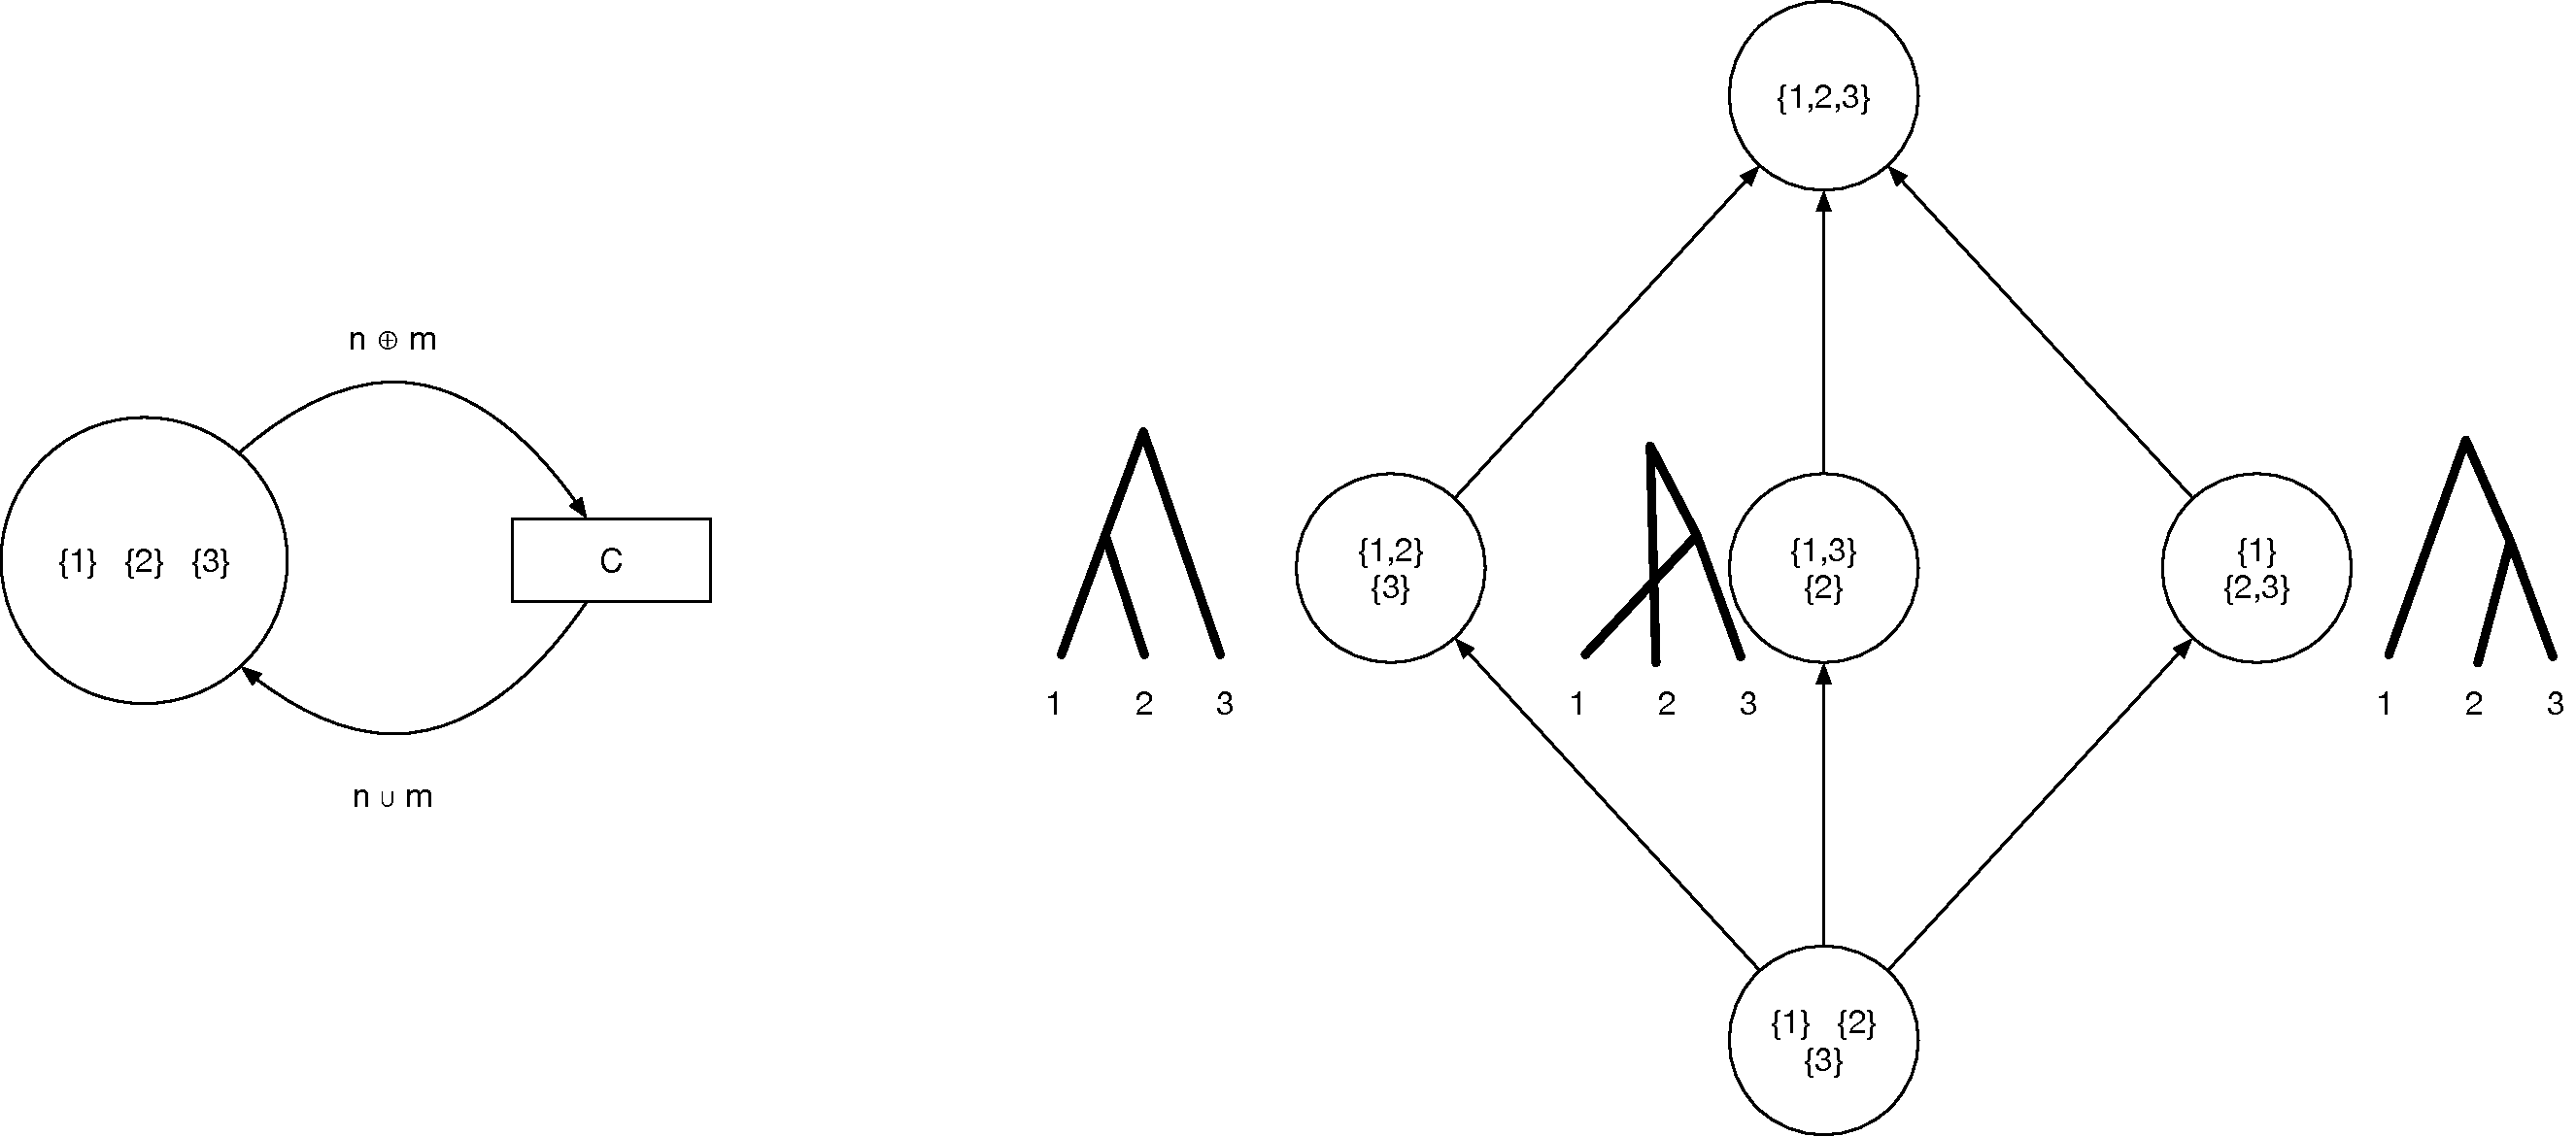
\includegraphics[scale=.25]{figures/coalescence-CPN}
\caption{Coalescence token game and state space for a setup with three initial genes. Each path through the reachability graph from the initial state to the final state, the bucket containing $\{1,2,3\}$ correspond to a topology of the genealogy of three genes. These topologies are shown next to the middle node in these paths. In actual runs of the coalescence CTMC, branch length probabilities are determined by the stochasticity of the CTMC.}
\label{fig:coalescence-CPN}
\end{figure}

The coalescence rate $C$ is traditionally not a primary parameter of the coalescence process. Rather, it is defined via the so-called ``effective population size'', $2N_e$, or its mutation-scaled version $\theta=4 N_e \mu$, see \citet{Hein:2004ta}, where $C=2/\theta$. Within the CTMC framework we use in this chapter, however, it is more convenient to use $C$ as the primary unit and the effective population size as the derived.


\subsubsection{Populations and migration}

We can consider modelling a slightly more complex scenario, one with several populations and migration between them. We can model this by tagging lineages with the population they are currently in on the tokens we represent them by. The tokens will then contain pairs of populations combined with sets representing lineages. We will only allow coalescences between lineages in the same population, so the coalescence transition must be updated to \trans{(p,n) \oplus (q,m)}{C}{(p_1,n\cup m)} when $p = q$. We can migrate by changing the population of a token to another, so use the transition \trans{(p,n)}{M}{(q,n)} where $p\neq q$.

Both these transitions assume the populations are symmetric---the coalescence transition assumes that the rate of coalescence is the same in all populations while the migration transition assumes that the migration rate between any pair of populations will be the same. This need not be the case, and by using different transitions we can introduce asymmetric migration, as shown in Fig.~\ref{fig:migration-coalescence-CPN}, where we have different rates for migration from a population 1 to a population 2 than from 2 to 1. We can do the same for modelling different coalescence rates in different populations, capturing that the populations might have different effective sizes, as shown in Fig.~\ref{fig:migration-coalescence-CPN-2} for two populations. Of course, these can be combined to have both asymmetric migration and different coalescence rates in different populations.


\begin{figure}[h]
\sidecaption
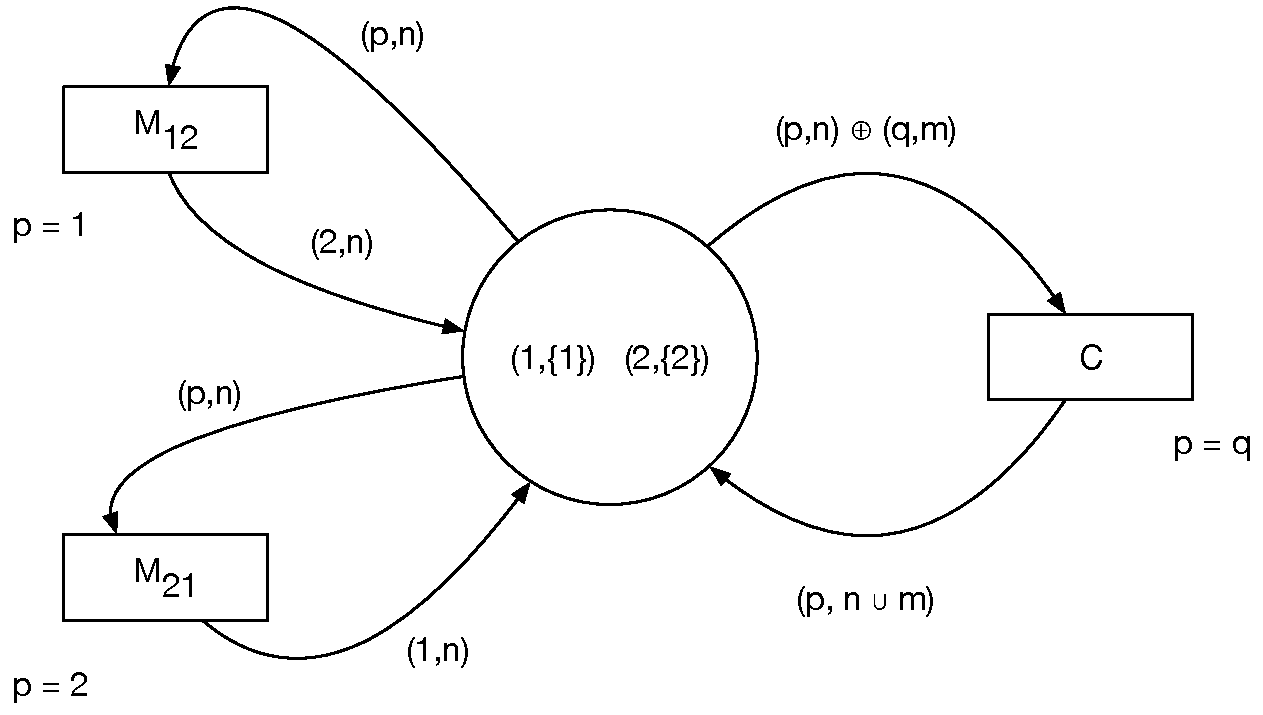
\includegraphics[scale=.30]{figures/migration-coalescence-CPN}
\caption{Token game for a coalescence process with two populations and (potentially asymmetric) migration between them.}
\label{fig:migration-coalescence-CPN}
\end{figure}

\begin{figure}[h]
\sidecaption
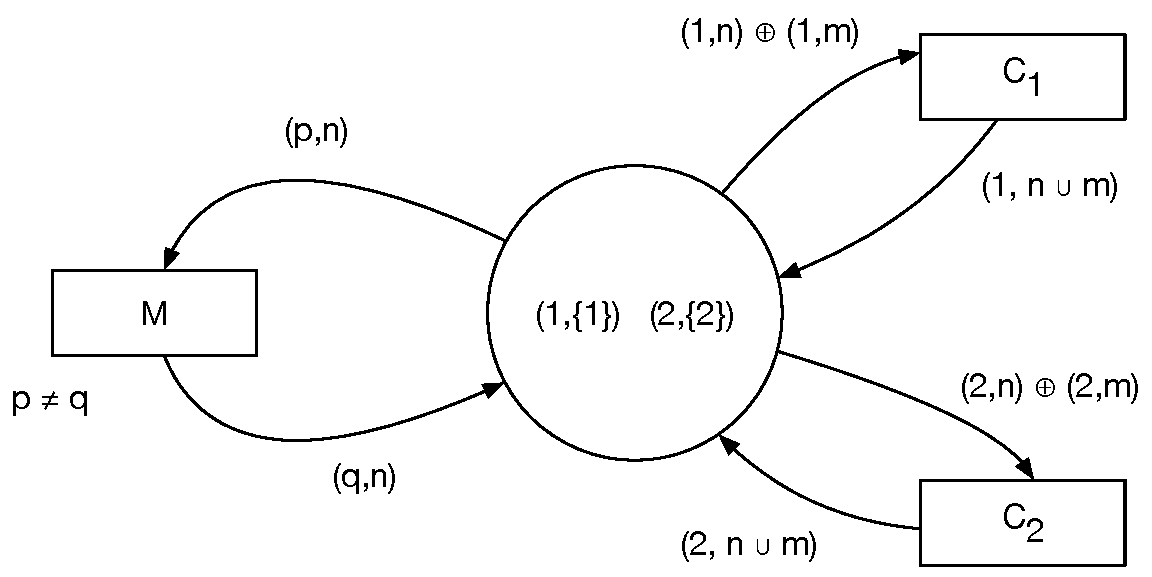
\includegraphics[scale=.30]{figures/migration-coalescence-CPN-2}
\caption{Token game for a coalescence process with two populations with symmetric migration between them but possibly different coalescence rates, i.e.\ different effective population sizes.}
\label{fig:migration-coalescence-CPN-2}
\end{figure}

Regardless of whether we use symmetric rates or not, the state space for the system with two populations and two samples will be the graph shown in Fig.~\ref{fig:migration-coalescence-state-space}. In this figure, the edges are labelled with rates assuming both asymmetric migration and different coalescence rates in the two populations. The separation between the upper two nodes and the lower four is caused by coalescence events. Migration events are reversible in the sense that you can migrate back and end up in the same state as before the event (at least when none of the migration rates are zero). Nodes connected only by migration transitions form what is known as \emph{strongly connected components}---subsets of the graph where all nodes are reachable from all others. Coalescence transitions, however, are not reversible. Whenever we move through a coalescence edge we end up in a part of the state space from which we can never reach the state we were in before the coalescence. This state space has two strongly connected components, the two top nodes and the four bottom nodes.

\begin{figure}[h]
\sidecaption
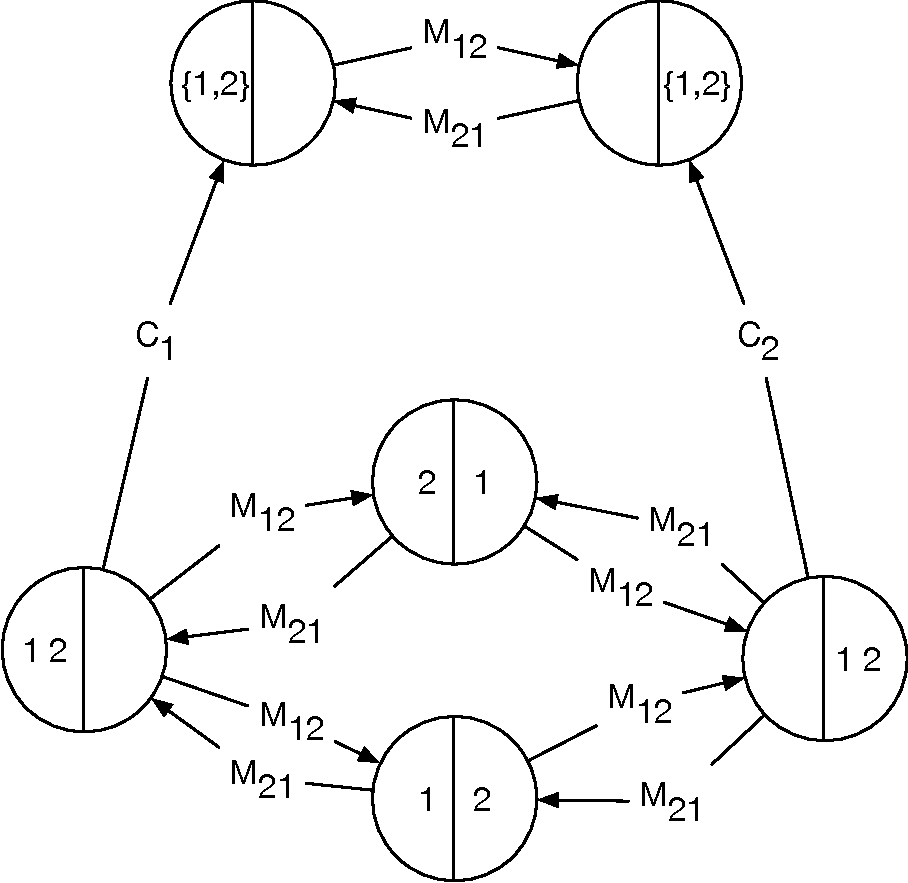
\includegraphics[scale=.30]{figures/migration-coalescence-state-space}
\caption{State space for the coalescence with population structure with two populations and two samples. We have changed the notation for the bucket slightly to improve readability, and tag lineages with populations by putting them to the left or to the right inside the bucket. We also show singleton sets as just their single element rather than in curly brackets.}
\label{fig:migration-coalescence-state-space}
\end{figure}

Figure~\ref{fig:migration-state-space-3} shows the state space graph for two populations and three initial samples. The space is substantially larger than for two samples---this is a general problem caused by combinatorial complexity known as the \emph{state space explosion} problem and is limiting problem for the methodology we construct here. However, we want you to notice the structure of strongly connected components and we have highlighted the five components in this graph using grey boxes.

\begin{figure}[t]
\sidecaption
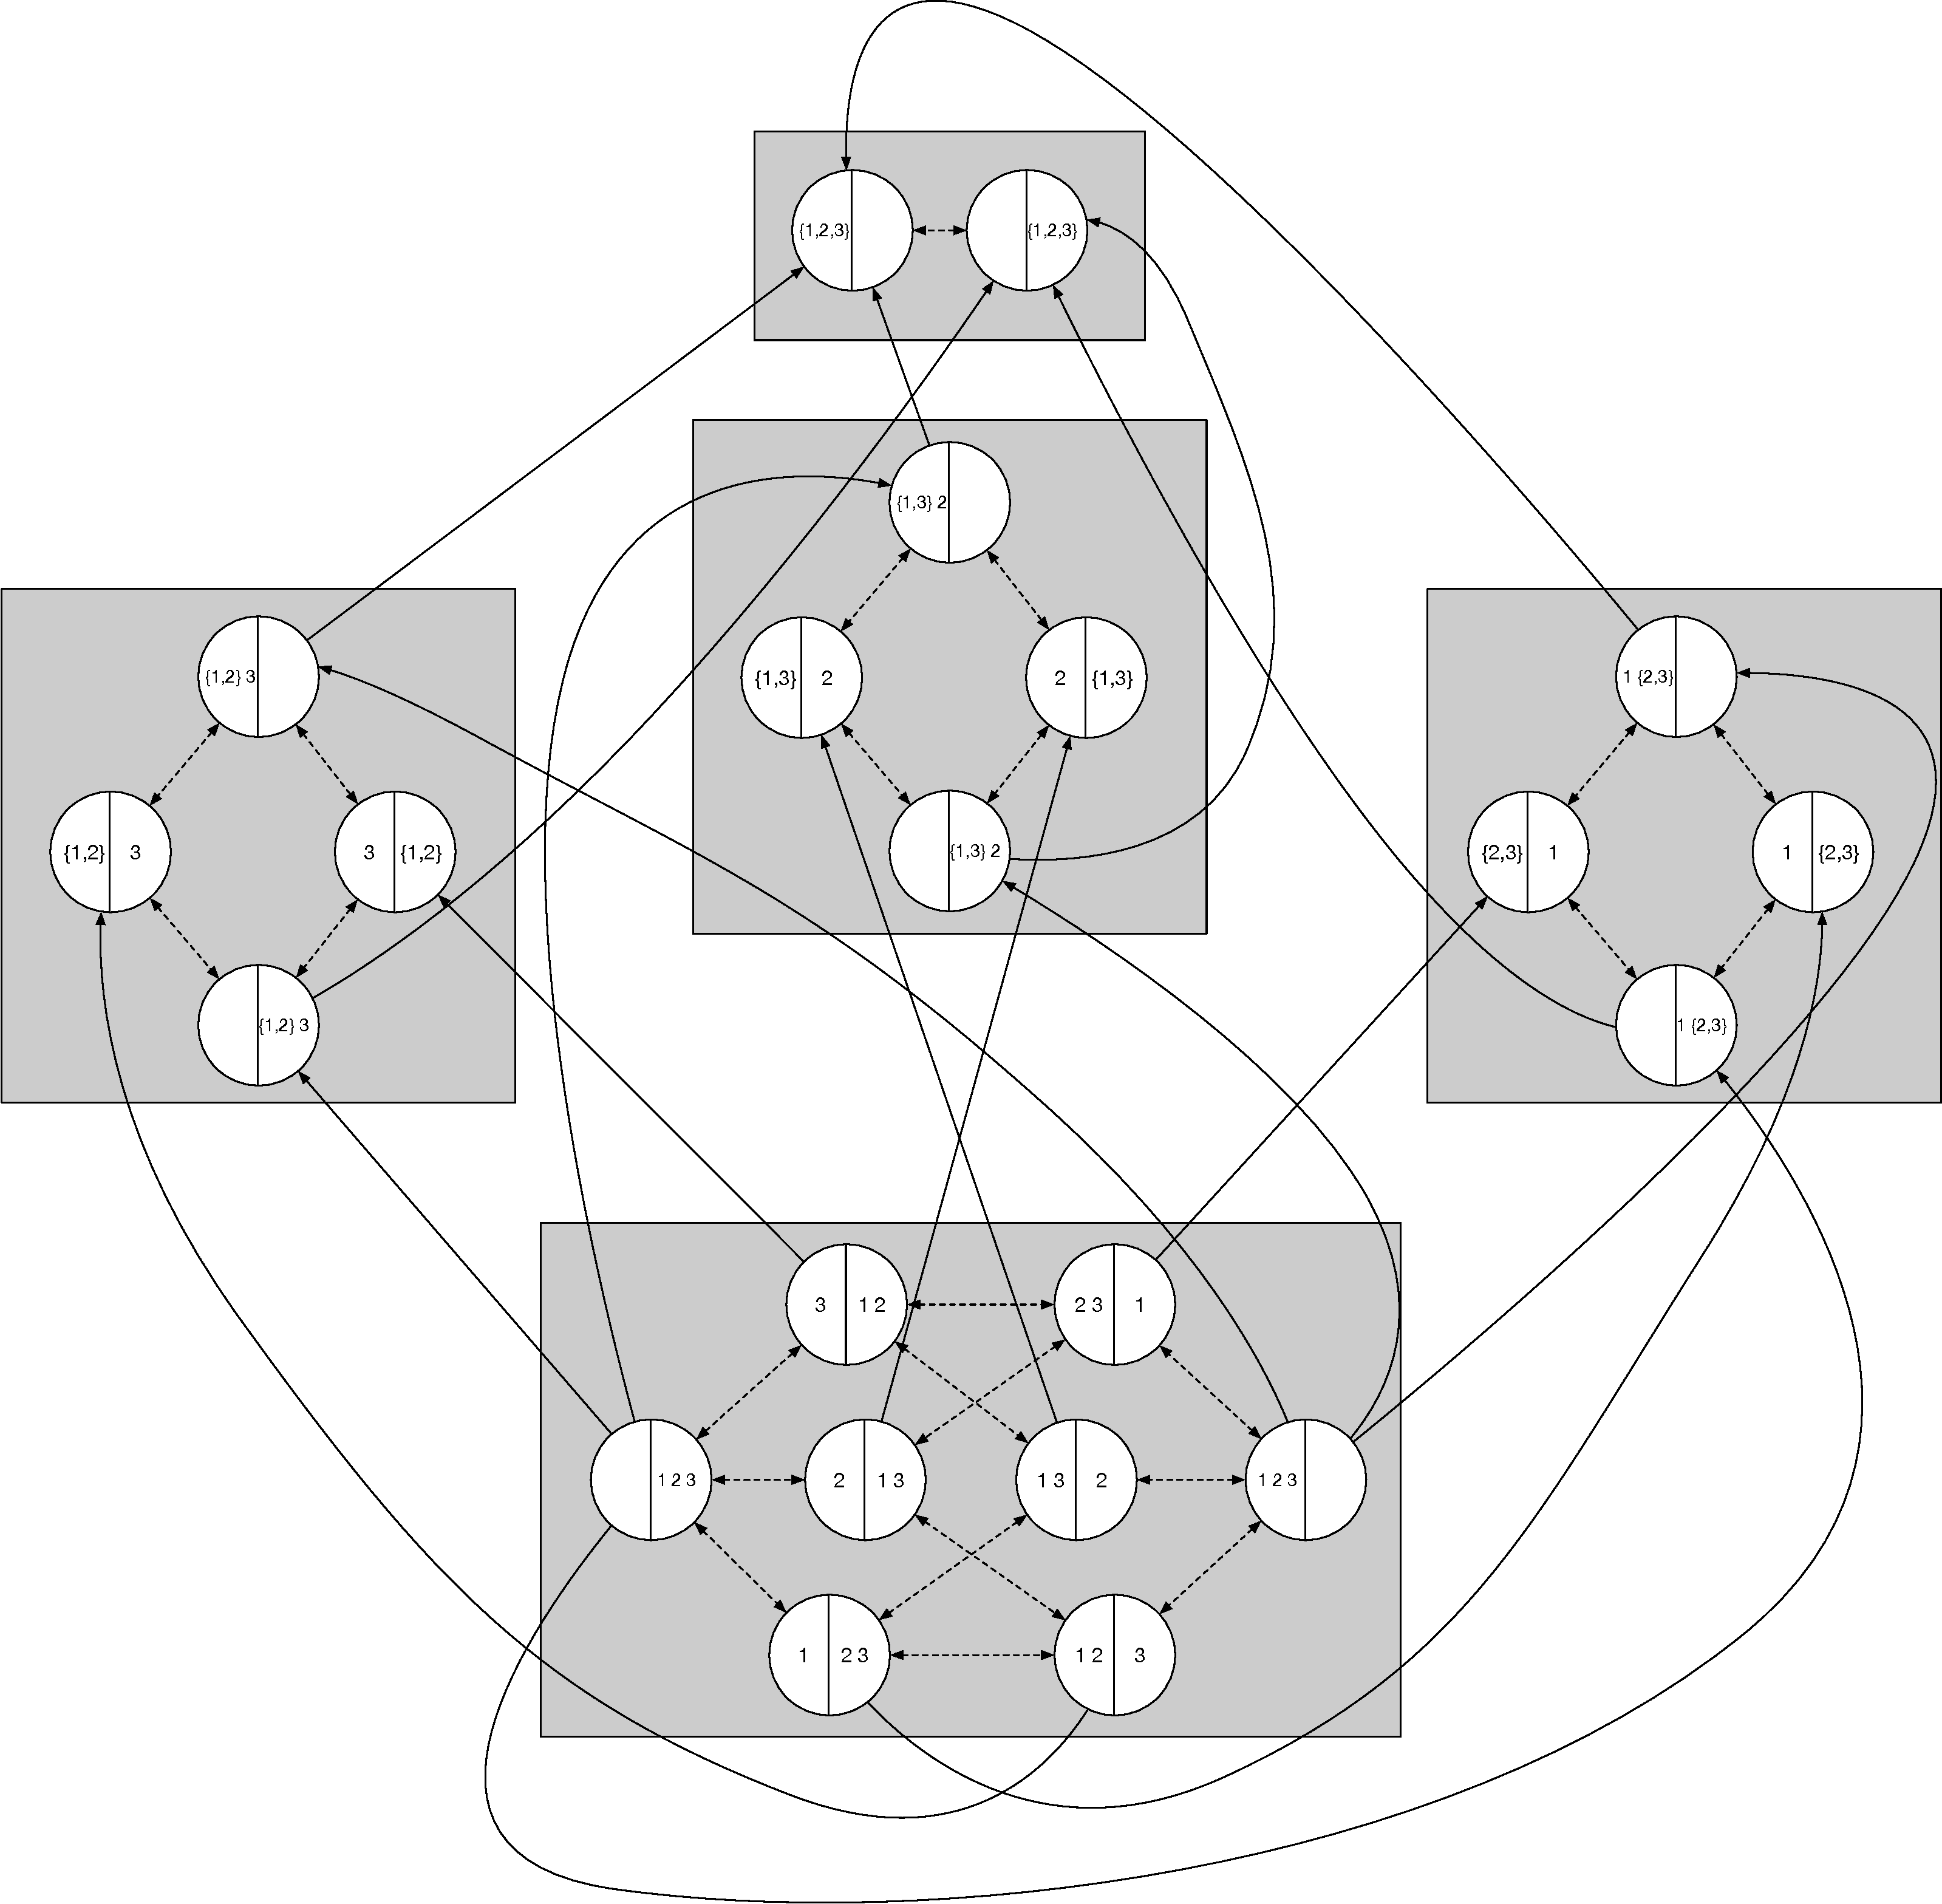
\includegraphics[scale=.20]{figures/migration-state-space-3}
\caption{State space for the coalescence with population structure with two populations and three samples. To ease readability we do not show edge labels and we show the reversible migration events as double-arrowed edges instead of two edges. Migration transitions are shown as dashed lines and coalescence transitions as solid lines.}
\label{fig:migration-state-space-3}
\end{figure}

We can construct a derived graph, the \emph{strongly connected component graph}, from such a state space. We use as nodes the strongly connected components in the original graph and we add an edge in the new graph between two components if there is an edge in the original graph going from a node in the first component to a node in the second. The strongly connected component graph for the graph in Fig.~\ref{fig:migration-state-space-3} is shown in Fig.~\ref{fig:migration-SCC-graph}. Notice that the graph is identical to the state space for three samples when we didn't have any migration (see Fig.~\ref{fig:coalescence-CPN}) and notice that genealogy topologies correspond to paths in this graph.

\begin{figure}[h]
\sidecaption
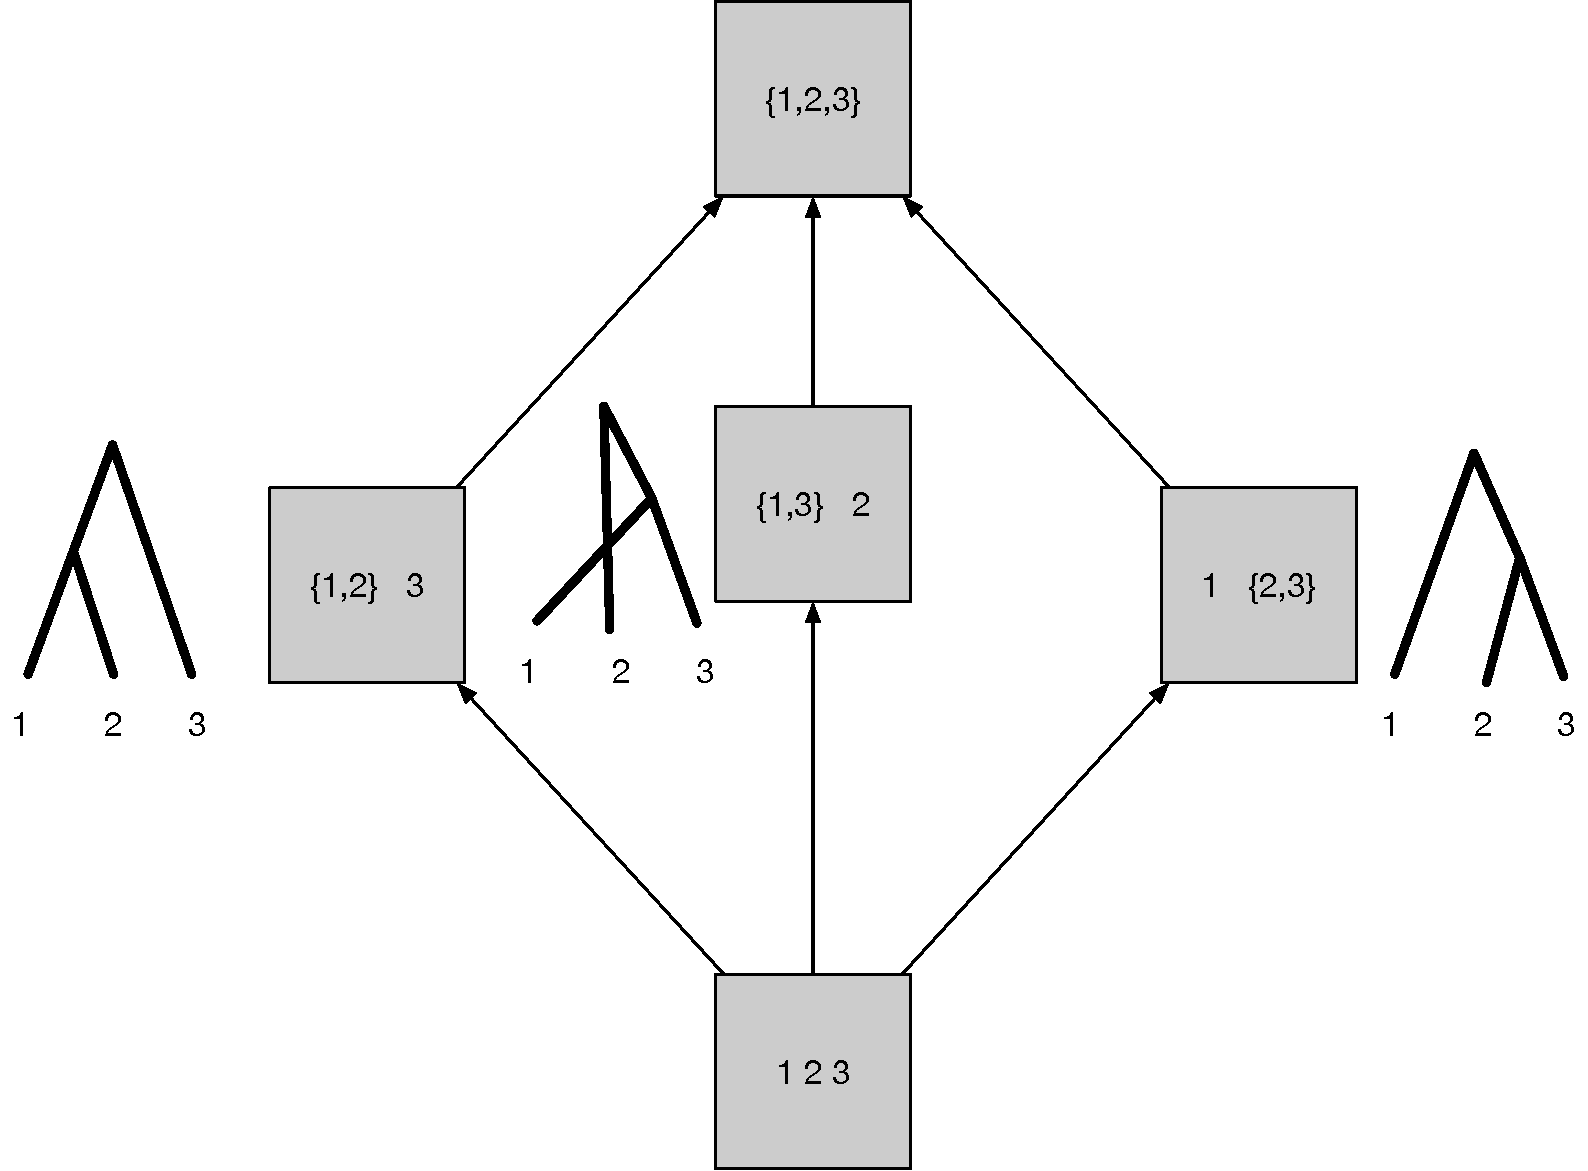
\includegraphics[scale=.20]{figures/migration-SCC-graph}
\caption{The strongly connected component graph for the migration system with three samples. Strongly connected components from the initial graph are shown as square boxes. Corresponding genealogies are shown next to the middle node of paths going from the initial component to the terminal component.}
\label{fig:migration-SCC-graph}
\end{figure}

Since the migration system contains reversible transitions, there will be events in a trace of the CTMC that will not be captured by the genealogy. At least not in the topology; we would expect the events to change the distribution of branch lengths but they would not change the topology. As long as the only irreversible transitions we have are coalescence transitions, however, we will have a one-to-one correspondence between genealogy topologies and paths in the strongly connected component graph from the initial component to the terminal component.


\subsubsection{The coalescent with recombination}

Going back to a single population, we can introduce recombination by adding structure to the genes we we hold in tokens. With recombination we consider genes as consisting of sequences of $L$ nucleotides.\footnote{In some formulations of the coalescence process with recombination, such as in \citet{Hein:2004ta}, genes are modelled as continuous segments. This simplifies some mathematics since recombinations can never occur at the exact same spatial point more than once, but it does not match real biology. In this chapter, we stick to discrete genes consisting of $L$ contiguous nucleotides.} In our tokens, we simply represent these as tuples of lineages. 

We need to modify the coalescence transition to capture this, and it becomes:
\begin{equation}
\trans{(n_1,n_2,\ldots,n_L) \oplus (m_1,m_2,\ldots,m_L)}{C}{(n_1\cup m_1,n_2\cup m_2,\ldots, n_L \cup m_L)}
\end{equation}

We also need to introduce a recombination transition which will split a lineage at some random index $k$, $1<k<L$, and produce two new lineages consisting of the first $k$ and last $L-k$ nucleotides, respectively, of the original lineage, so:
\begin{equation}
\trans{(n_1,n_2,\ldots,n_L)}{R_g}{(n_1,\ldots,n_k,\emptyset,\ldots,\emptyset)\oplus(\emptyset,\ldots,\emptyset,n_{k+1},\ldots,n_L)}
\end{equation}
for some $k$ and where $R_g$ is the per-gene recombination rate (which is $R_g=(L-1)R_n$ if $R_n$ is the per-nucleotide recombination rate).

This formulation is not perfect since it can produce lineages with no ancestral material, and an arbitrary number of these, so the state space is infinite. We can fix this by not allowing recombinations that leaves such lineages, but this requires us to adjust the rate and we need different transitions for all pairs of indices:
\begin{equation}
\trans{(\emptyset,\ldots,\emptyset,n_i,\ldots,n_j,\emptyset,\ldots,\emptyset)}{(j-i)R_n}{(n_1,\ldots,n_k,\emptyset,\ldots,\emptyset)\oplus(\emptyset,\ldots,\emptyset,n_{k+1},\ldots,n_L)}
\end{equation}
where $i<k<j$ and $n_i\neq\emptyset$ and $n_j\neq\emptyset$.

We are not interested in length $L$ genes, however, since we aim to model only two neighbouring nucleotides, so we will only work with pairs. We will therefore use $R$ as the per-nucleotide recombination rate (actually, the rate at which we break apart a pair) and have the two transitions shown in Fig.~\ref{fig:coalescence-recombination-CPN}.

\begin{figure}[h]
\sidecaption
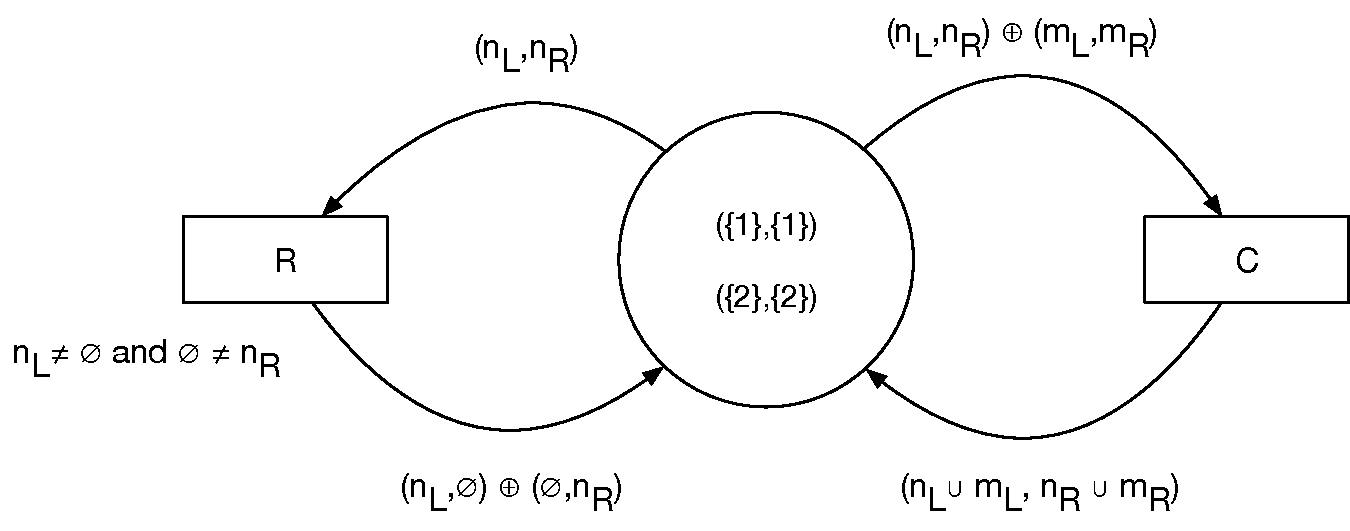
\includegraphics[scale=.30]{figures/coalescence-recombination-CPN}
\caption{Token game for coalescence with recombination for pairs of nucleotides. The condition on the recombination transition ensures that we never produce lineages with no ancestral material.}
\label{fig:coalescence-recombination-CPN}
\end{figure}


\subsubsection{Genealogies and CTMC traces}

\todo[inline]{Everything after this point needs to be rewritten to match the graphical language of CTMC construction}


\subsection{Changing demographics and chaining CTMCs}
\todo[inline]{I can get some bits and pieces from the old section for this that I have left below.}

\subsection{Constructing coalescent hidden Markov models}

\todo[inline]{Update this intro. I stole from it for an earlier section}

To construct a hidden Markov model to approximate the coalescence process for a given demographic model, with a given set of associated parameters, we must construct the HMM parameters: the tuple $(\pi,\T,\E)$. As seen in \eqref{eq:pi-from-joint-prob} and \eqref{eq:transitions-from-joint-prob}, we can derive $\pi$ and $\T$ from joint probabilities of two genealogies, and as mentioned earlier, we can compute $\E$ from standard algorithms (once we have discretised time), so the crux of deriving the CoalHMM is computing probabilities $\Pr(G_i,G_{i+1})$. This, we can compute from the CTMC that models the coalescence process in the given demography; if we know how the CTMC that models the lineages of two neighbouring nucleotides change over time, we can extract the two neighbouring genealogies from it.

We need a finite number of genealogies to construct a finite $\pi$ vector and a finite $\T$ matrix, so we first discretise time. Let $(\tau_1=0,\tau_2,\ldots,\tau_m)$ be $m$ time points with $\tau_i<\tau_{i+1}$. We discretise time by only considering the CTMC states at these specific time points. Any coalescences that occur between two of these points we place at a time point $\sigma_i: \tau_i < \sigma_i < \tau_{i+1}$ for $1 \leq i < m$ and if we have lineages that haven't found their most recent common ancestor at time $\tau_{m}$ we assume they happen at a $\sigma_m > \tau_m$. There are multiple ways to pick both time points $\tau_i$ and $\sigma_i$; in our software we use heuristics described in \citet{Mailund:2011dva} and \cite{Mailund:2012ewa}, but as the number of time points increase, so the discretisation gets finer, the choice of discretisation gets less important.

With this discretisation, we can define a genealogy by which partitions of lineages we have at each of the $\tau_i$ time points: a \emph{genealogy} $G$ is a sequence of partitions of lineages, $(p_1,p_2,\ldots,p_m)$, such that each lineage in $p_i$ can be formed from the union of one or more lineages in $p_{i-1}$. Now, given two such genealogies, $G$ and $G'$, with partitions at the $m$ $\tau_i$ points $(p_1,p_2,\ldots,p_m)$ and $(p'_1,p'_2,\ldots,p'_m)$, we want to know the joint probability $\Pr(G_i=G,G_{i+1}=G')$. We can \emph{almost} get this from a CTMC modelling the coalescence process. If we denote the CTMC by $\left\{ X(t) \,|\, t\geq 0 \right\}$, then we can compute the likelihood that it is in specific states at each $\tau_i$ as this,
\begin{equation}
	\Pr(X(\tau_1)=x_1,X(\tau_2)=x_2,\ldots,X(\tau_m)=x_m) =
	\prod_{i=1}^{m-1} \exp\left(Q\left(\tau_{i+1}-\tau_i\right)\right)_{x_i,x_{i+1}}
\end{equation}
where $Q$ is the rate matrix for the CTMC. The states in the CTMC, however, contain more information than what we can see from the two genealogies. The states in the CTMC contain information about which lineages on the left genealogy are linked to which lineages on the right genealogy. If we only know which lineages are in the left and which are in the right genealogy at any given $\tau_i$ time point, we do not have this information.

Consider the simplest non-trivial example of two samples from one population. Its states are shown in Table~\ref{tbl:psmc-like-ctmc}, where black dots at the top and bottom refers to sample one and two, respectively, and white circles refer to common ancestors. Lines between lineages on the left and right indicates that the left and right nucleotides are linked, i.e.\ on the same chromosome, while the absence of lines indicate that they are not. It is the CTMC we can define by starting in state $\{(\{1\},\{1\}),(\{2\},\{2\})\}$ and following the rules\todo{Should we define transition systems earlier and refer to that here, or keep at this semi-formal/informal level?}
\begin{itemize}
	\item $\{(l_1,r_1)\}\cup\{(l_2,r_2)\}\cup\text{Rest} \overset{C}{\to}\{(l_1\cup l_2,r_1 \cup r_2)\}\cup\text{Rest}$ 
	\item $\{(l,r)\}\cup\text{Rest} \overset{R}{\to} \{(l,\emptyset)\}\cup\{(\emptyset,r)\}\cup\text{Rest}$ if $l\neq\emptyset$ and $r\neq\emptyset$.
\end{itemize}
Read the first rule as lineage $(l_1,r_1)$ coalesces with lineage $(r_1,r_2)$ at rate $C$ while leaving the rest of the lineages unchanged. Read the second as the lineage $(l,r)$ recombining at rate $R$, while leaving the rest of the lineages unchanged, but only if both $l$ and $r$ are non-empty, i.e.\ as long as we have ancestral material both to the left and to the right of the recombination point.

\begin{table}[tb]
  \caption{CTMC states for two samples in the same population.}
  \label{tbl:psmc-like-ctmc}
  \centering
  \scalebox{.7}{
  \begin{tabular}{c|c|c|c|c|c|c|c|c|c|c|c|c|c|c|c}
    Index & 1 & 2 & 3 & 4 & 5 & 6 & 7 & 8 & 9 & 10 & 11 & 12 & 13 & 14 & 15\\ \hline
    State & 
    % 1
    $\xymatrix @R=0.5pc @C=0.5pc {
      \bullet & \bullet \\
      \bullet & \bullet }$ & 
    % 2
    $\xymatrix @R=0.5pc @C=0.5pc {
      \bullet \ar@{-}[r] & \bullet \\
      \bullet & \bullet }$ &
    % 3
    $\xymatrix @R=0.5pc @C=0.5pc {
      \bullet & \bullet \\
      \bullet \ar@{-}[r] & \bullet }$ &
    % 4
    $\xymatrix @R=0.5pc @C=0.5pc {
      \bullet \ar@{-}[r] & \bullet \\
      \bullet \ar@{-}[r] & \bullet }$ &
    % 5
    $\xymatrix @R=0.5pc @C=0.5pc {
      \bullet \ar@{-}[dr] & \bullet \\
      \bullet  & \bullet }$ &
    % 6
    $\xymatrix @R=0.5pc @C=0.5pc {
      \bullet  & \bullet \\
      \bullet \ar@{-}[ur] & \bullet }$ &
    % 7
    $\xymatrix @R=0.5pc @C=0.5pc {
      \bullet \ar@{-}[dr] & \bullet \\
      \bullet \ar@{-}[ur] & \bullet }$ &

    % 8
    $\xymatrix @R=0.1pc @C=0.5pc {
            & \bullet \\
      \circ &  \\
            & \bullet }$ &
    % 9 
    $\xymatrix @R=0.1pc @C=0.5pc {
                    & \bullet \\
   {\circ} \ar@{-}[ur] & \\
                    & \bullet }$ &    
    % 10
    $\xymatrix @R=0.1pc @C=0.5pc {
      & \bullet \\
      \circ \ar@{-}[dr] &\\
      & \bullet} $ &

    % 11 
    $\xymatrix @R=0.1pc @C=0.5pc {
      \bullet & \\
      & \circ  \\
      \bullet} $ &
    % 12
    $\xymatrix @R=0.1pc @C=0.5pc {
      \bullet \ar@{-}[dr] &  \\
      & \circ\\
      \bullet }$ &
    % 13
    $\xymatrix @R=0.1pc @C=0.5pc {
      \bullet &  \\
      & \circ \\
      \bullet \ar@{-}[ur] }$ &
      
    % 14
    $\xymatrix @R=0.5pc @C=0.5pc {
      \circ \ar@{-}[r] & \circ }$ &
    % 15
    $\xymatrix @R=0.5pc @C=0.5pc {
      \circ & \circ }$ \\ \hline
    Classes & \multicolumn{7}{c|}{$N$} &
    \multicolumn{3}{c|}{$L$} &
    \multicolumn{3}{c|}{$R$} &
    \multicolumn{2}{c}{$B$}
  \end{tabular}
  }
\end{table}


The transition rules define not only the state space of the CTMC but also the its rate matrix. All non-diagonal cells will be rates equal to one of $C$, $R$, or zero. Entry $Q_{i,j}$ will be $C$ when you can get from state $i$ to state $j$ following the first rule, $R$ when you can get from $i$ to $j$ by following the second rule. If there are no direct rule to get you from $i$ to $j$, the instantaneous rate, and thus $Q_{i,j}$, is zero. The rate matrix looks like this:
\begin{equation}
  \label{eq:two-samples-ctmc}
  Q = 
\begin{blockarray}{lccccccccccccccc}
	\quad\;\;
 & \BAmulticolumn{7}{c}{N} & \BAmulticolumn{3}{c}{L} & \BAmulticolumn{3}{c}{R} & \BAmulticolumn{2}{c}{B} \\
\begin{block}{l(ccccccc|ccc|ccc|cc)}
  & - & C & C &   & C & C &   & C &   &   & C &   &   &   &   \\
  & R & - &   & C &    &     &   &   & C &   &   & C &   &   &   \\
  & R &   & - & C &   &   &   &   &  & C &   &   & C &   &   \\
  N &   & R & R & - &   &   &   &   &  &   &   &   &   & C &   \\ 
  & R &   &   &   & - &   & C &  &   & C &   & C &   &   &   \\
  & R &   &   &   &   & - & C &   & C &   &   &   & C &   &  \\
  &   &   &   &   & R & R & - &   &   &   &   &   &   & C &   \\
  \BAhhline{&---------------}
   & &   &   &  &   &   &   & - & C & C &   &   &   &   & C \\
  L & &   &   &  &   &   &   & R & - &   &   &   &   & C &   \\
   & &   &   &  &   &   &   & R &   & - &   &   &   & C &   \\ 
  \BAhhline{&---------------}
   & &   &   &  &   &   &   &   &   &   & - & C & C &   & C \\
  R & &   &   &  &   &   &   &   &   &   & R & - &   & C &   \\
   & &   &   &  &   &   &   &   &   &   & R &   & - & C &   \\ 
  \BAhhline{&---------------}
  B & &   &   &  &   &   &   &   &   &   &   &   &   & - & R \\
   & &   &   &  &   &   &   &   &   &   &   &   &   & C & - \\
\end{block}
\end{blockarray}
\end{equation}

If we only know the lineages that exists at the left and right nucleotide, respectively, there are equivalence classes of states that we cannot distinguish. In the table and the matrix these are named $N$ (for no MRCA), $L$ (for when only the left nucleotide has reached the MRCA), $R$ (for when only the right nucleotide), and $B$ (for when both have). If we know the the left and right genealogies, we will know for each time point $\tau_i$ which class the CTMC state is in, but not the exact state. To compute the probability of two genealogies, we need to sum over the states in each equivalence class.


For a two-nucleotide CTMC, each lineage is a pair of (possibly empty) sets of initial samples. If we extract the left or right nucleotides of all lineages in a CTMC state $s$, we would in both cases get a partitioning of the original samples---call those $l(s)$ and $r(s)$, respectively. It is these pairs that define the equivalence classes; any two states $s$ and $s'$ with $l(s)=l(s')$ and $r(s)=r(s')$ are equivalent. For the simple case we have just considered, $N$ is the equivalence class defined by $l=\{\{1\},\{2\}\}$ and $r=\{\{1\},\{2\}\}$, $L$ has $l=\{\{1,2\}\}$ and $r=\{\{1\},\{2\}\}$, $R$ has those partitions flipped, and $B$ has both $l=\{\{1,2\}\}$ and $r=\{\{1,2\}\}$.

For a pair of genealogies $G=(p_1,p_2,\ldots,p_m)$ and $G'=(p'_1,p'_2,\ldots,p'_m)$, pairing them up component wise gives is a sequence of CTMC equivalence classes $(c_1=(p_1,p'_1),c_2(p_2,p'_2),\ldots,c_m=(p_m,p'_m))$. The joint probability of the two genealogies can then be obtained from the CTMC as this:
\begin{eqnarray}
	\Pr(G_i=G,G_{i+1}=G') &=& 
	\Pr(X(\tau_1)\in c_1,X(\tau_2)\in c_2,\ldots,X(\tau_m)\in c_m) \\
	&=& 
	\label{eq:ctmc-probability-of-joint-genealogies}
	\sum_{x_1\in c_1}\sum_{x_2\in c_2}\cdots\sum_{x_m\in c_m}
	\prod_{i=1}^{m-1} \exp\left(Q\left(\tau_{i+1}-\tau_i\right)\right)_{x_i,x_{i+1}}
\end{eqnarray}
and the sum and products can be rearranged---similar to how it is done for hidden Markov models---to produce a dynamic programming algorithm that lets us computed the joint probability efficiently.

While this framework might seem complicated, from \eqref{eq:ctmc-probability-of-joint-genealogies} it should be obvious that we can automatically derive a CoalHMM as long as we have the rate matrix of a CTMC modelling the demography of interest, $Q$, and a discretisation of time $(\tau_1,\ldots,\tau_m)$.


\subsection{Modelling demography as sequences of CTMCs}

To actually capture demographies, we must make two slight changes to \eqref{eq:ctmc-probability-of-joint-genealogies}; the first allows us to vary parameters of the demography for different time periods and the second allows us to model population changes, such as moving from isolation periods to migration periods, to split populations into descendant populations, or model admixture events. Equation \eqref{eq:ctmc-probability-of-joint-genealogies} uses the same rate matrix in all time intervals, but this assumes no demographic changes. The first modification we do is to associate each time interval with its own rate matrix:
\begin{equation}
	\Pr(G_i=G,G_{i+1}=G') =
	\prod_{i=1}^{m-1} \exp\left(Q_i\left(\tau_{i+1}-\tau_i\right)\right)_{x_i,x_{i+1}}
	.
\end{equation}

In practise, we cannot have distinct rate matrices for each time interval; we would not be able to infer the parameters if we did. Instead, we use the same matrix for some consecutive intervals, as was done with Li and Durbin's PSMC model for inferring changes to effective population sizes over time \cite{Li:2011eza}. Since effective population sizes are inversely proportional to coalescence rates, in order to implement PSMC in the framework we have just presented, we would only need to modify the rate matrix in \eqref{eq:two-samples-ctmc} such that the coalescence rate $C$ depends on which time interval we consider.

A CTMC that models two populations and allow migration of lineages between them can be constructed in a similar way \cite{Mailund:2012ewa} and by varying migration rates between different time intervals, we can infer changes to migration rates over time \cite{Cheng:2015kia} (although with less inference accuracy). 

To model multiple populations, we tag each lineage with which population it is in. Instead of representing lineages as pairs of left and right nucleotides, we represent them as triplets $(p,l,r)$ of population, left and right nucleotide.

We modify the two transition rules we saw before to include population information and to only allow coalesce events between lineages lineages in the same population:
\begin{itemize}
	\item $\{(p_1,l_1,r_1)\}\cup\{(p_2,l_2,r_2)\}\cup\text{Rest} \overset{C}{\to}\{(p_1,l_1\cup l_2,r_1 \cup r_2)\}\cup\text{Rest}$ if $p_1=p_2$
	\item $\{(p,l,r)\}\cup\text{Rest} \overset{R}{\to} \{(p,l,\emptyset)\}\cup\{(p,\emptyset,r)\}\cup\text{Rest}$ if $l\neq\emptyset$ and $r\neq\emptyset$.
\end{itemize}
If we want to allow (continuous) migration from population $i$ to $j$ (when going back in time, i.e.\ from $j$ to $i$ when going forward in time), we add the rule
\begin{itemize}
	\item $\{(p_i,l,r)\}\cup\text{Rest} \overset{M_{i,j}}{\to} \{(p_j,l,r)\}\cup\text{Rest}$.
\end{itemize}
We can add rules for migrations between any pair of populations and make the rates symmetric or asymmetric.

In practise, the state space of the CTMC grows very quickly with more populations, so we have only worked with two populations in practise. In \citet{Mailund:2012ewa} with a single, symmetric, migration between the populations and in \citet{Cheng:2015kia} with a few periods of different rates.

We can combine isolation models---where lineages cannot move from one population to another---with migration models---where they can, by setting migration rates to zero in some time intervals. We cannot, however, construct the isolation model of \citet{Mailund:2011dva} or the isolation with initial migration model of \citet{Mailund:2012ewa} just by modifying rates in the same rate matrix. Both models have two populations in the presence, but at some point in the past, those split from an ancestral population. Tracing lineages back in time, the CTMC must at some instantaneous time-point move all lineages to this ancestral population.

In general, we can have different CTMCs with different state spaces before and after time $\tau_i$. To deal with this, we introduce a matrix $\eta^i$ that maps from the state space immediately before $\tau_i$ to the state space immediately after. The entry $\eta^i_{s,t}$ should be the probability that state $s$ maps to state $t$. We use this $\eta^i$ to modify \eqref{eq:ctmc-probability-of-joint-genealogies} to
\begin{equation}
	\Pr(G_i=G,G_{i+1}=G') = 
	\sum_{x_1\in c_1}\sum_{x_2\in c_2}\cdots\sum_{x_m\in c_m}
	\prod_{i=1}^{m-1} \left[\exp\left(Q\left(\tau_{i+1}-\tau_i\right)\right)\eta^i\right]_{x_i,x_{i+1}}
\end{equation}


There are some restrictions on $\eta^i$ since we want to ensure that each original sample is preserved in some ancestral lineage with probability one on both the left and the right nucleotides. One way to ensure this is to construct the matrix from a mapping of individual lineages.

Consider the model from \citet{Mailund:2012ewa}\todo{add a figure for the model}\ that has an initial period with two populations and no migration between them, followed (when looking back in time) by a period with migration, and at last a third period in an ancestral population. We will model lineages as triplets $(p,l,r)$ and consider there to be three populations, $p_1$, $p_2$ and $p_A$ where $p_A$ is the ancestral population. In the first period, we do not allow migration, so at the instant we move from that period to the one where we do, all lineages will be in the same population they started in. The lineage $(p,l,r)$ will map to $(p,l,r)$ with probability one. It looks a little like nothing changes, but the state spaces actually do. There are more possible states in the second period than in the first. When considering the entire state of the CTMC, it consists of a set of lineages, and each map to one other lineage---itself but in the other state space---so the resulting state is the set you get by mapping all the elements in the first state. The mapping $\eta$ is an injection. It maps each point in a subset of the second state space to itself.

When we move from the second to the third period, all lineages should change their population to $p_A$, so $(p,l,r)\mapsto(p_A,l,r)$ with probability one for all lineages. Again, we derive the mapping from state to state from this mapping between lineages by just applying the mapping to each lineage in each state. This $\eta$ is slightly different than the first since this one maps from a larger state space into a smaller. It is more like a projection than an injection. For both mappings, each state maps to one unique other state with probability one, but for the second mapping, several input states will map to the same output state.

We will not always map each state to a single other state with probability one; sometimes there is a distribution of states we map to. Consider an admixture event where two populations, $p_1$ and $p_2$, admix to become population $p_3$.\todo{Make a figure for this}\ If $p_3$ is created with fraction $\alpha$ of its population from $p_1$ and $1-\alpha$ from $p_2$, then a lineage $(p_3,l,r)$ will map to $(p_1,l,r)$ with probability $\alpha$ and to $(p_2,l,r)$ with probability $1-\alpha$. The probabilities associated with which lineages map to which carries over to states. State $s$ maps to state $t$ with probability $P$ if $t$ is the result of mapping the individual lineages in $s$ and $P$ is the product of the individual lineage mappings used.\todo{Give an admixture example}



\section{Using Jocx, a CoalHMM inference tool}
\todo[inline]{This is probably where we should describe that we only look at pairs and then use a composite likelihood}
\todo[inline]{Tutorial in how to use the software}

\section{CoalHMM results (better title)}
\todo[inline]{Some simulation results}


\bibliographystyle{spbasic}
\bibliography{references.bib}

\end{document}
